\chapter{Introduction to FCS}
\label{sec:IntroductionToFCS}
\begin{center}
  \itshape \underline{Note:} This section is in part copied (and adapted) from my PhD thesis \cite{KRIEGERPHD2014}!
\end{center}

\noindent The software \df has been developed to simulate \itindex{fluorescence correlation spectroscopy} (\itindex{FCS}) and \itindex{fluorescence cross-correlation spectroscopy} (\itindex{FCCS}) measurements, based on particle trajectories.

\section{Introduction to fluorescence correlation spectroscopy}
\label{sec:IntroductionToFluorescenceCorrelationSpectroscopy}

\begin{figure}[b!]
	\centering
		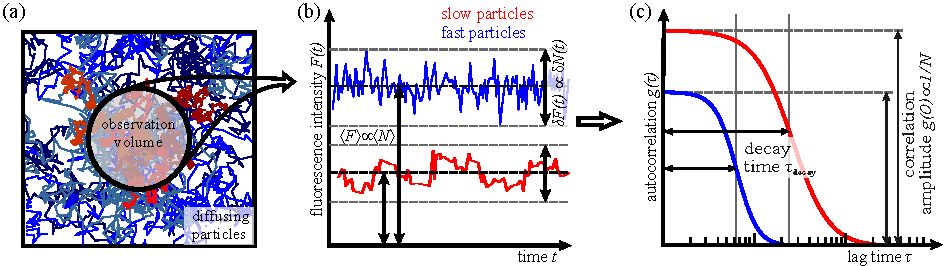
\includegraphics{pic/fcs_principle.pdf}
	\mycaption{Illustration of the principle of FCS.}{(a) Sample with particles moving with different diffusion coefficients (fast: blue, slow: red). The circle indicates the observation volume. (b) Fluorescence intensity, as measured from the sample in (a), showing the fluorescence fluctuations $\delta F(t)$ around the mean intensity $\mean{F}$. (c) Autocorrelation functions $g(\tau)$, calculated from the intensity traces in (b). The decay times $\taudecay$ are defined by $g(\taudecay)=g(0)/2$. }
	\label{fig:fcs_principle}
\end{figure}

FCS was introduced  in 1974 by \citeauthor*{MAGDE1974} in Refs.~\cite{MAGDE1974, MAGDE1974a,MAGDE1978}. As shown in \figref{fig:fcs_principle}, fluorescence is excited and detected in a tiny subvolume (a few $\unit{\mu m^3}$) of the sample containing only few particles $N(t)$ at any time. The measured fluorescence intensity $F(t)$ is proportional to this particle number. Due to the diffusive motion of the particles, $N(t)$ is permanently fluctuating around its mean value $\mean{N}$. This is represented as:
\begin{equation}\label{eq:fcs_particlenumber}
  N(t)=\mean{N}+\delta N(t)\ \ \ \ \ \Rightarrow\ \ \ \ \ F(t)=\mean{F}+\delta F(t)\ \ \ \ \ \text{with}\ \ \smean{\delta N(t)}=\smean{\delta F(t)}=0.
\end{equation}
Here $\delta N(t)$ and $\delta F(t)$ represent the fluctuations of the particle number and the fluorescence intensity. Depending on the speed of motion (diffusion coefficient), the particle number fluctuates ``faster'' or ``slower''. This can be quantified using an autocorrelation analysis. The normalized FCS autocorrelation function is defined as
\begin{equation}\label{eq:fcs_acf}
  g(\tau)=\frac{\mean{\delta F(t)\cdot\delta F(t+\tau)}}{\mean{F}^2}=\frac{\mean{ F(t)\cdot F(t+\tau)}}{\mean{F}^2}-1,\ \ \ \tau>0.
\end{equation}
where the averaging operation $\mean{\cdot}$ is defined as a a time average:
\begin{equation}\label{eq:fcs_avg}
  \mean{F(t)}=\lim\limits_{T\rightarrow\infty}\frac{1}{T}\cdot\int\limits_0^TF(t)\;\ddt.
\end{equation}
The autocorrelation function $g(\tau)$ measures the similarity of the signal $F(t)$ to its time-shifted version $F(t+\tau)$. If the fluctuations are completely random white noise, the correlation function is $g(\tau)\propto\ddelta(\tau)$, which is $0$ for all time lags $\tau>0$. If $F(t)$ contains a non-random component, the correlation will be non-zero over a lag-time range, which is characteristic for the non-random process. In FCS the non-random fluctuations are caused by Brownian motion of fluorescent particles, which implies a typical dwell time of the particles in the observation volume of\footnote{This equation is related to the mean-squared displacement (MSD) of a particle undergoing \itindex{normal diffusion}, which was shown by Albert Einstein to be $\langle r^2\rangle(\tau)=2\cdot d\cdot D\cdot\tau$, where $d$ is the dimensionality of the motion and $D$ is the \itindex{diffusion coefficient}.}:
\begin{equation}\label{eq:fcs_taudecay}
  \tauD\propto\frac{\left(\sqrt[3]{\Vobs}\right)^2}{D}.
\end{equation}
During this time, the presence of a single particle causes a self-similarity in the fluctuations, which manifests itself as a decay of the autocorrelation function from a zero-lag amplitude $g(0)>0$ to $g(\infty)=0$. The half-life time $\taudecay$ of this decay is approximately given by $\tauD$ from \eqref{eq:fcs_taudecay}.

The zero-lag amplitude $g(0)$ of the autocorrelation function \eqref{eq:fcs_acf} yields the average particle number in the observation volume, as
\begin{equation}\label{eq:fcs_acfn}
  g(0)=\frac{\smean{\delta F^2(t)}}{\mean{F}^2}\propto\frac{\smean{\delta N^2(t)}}{\mean{N}^2}=\frac{1}{\mean{N}}.
\end{equation}
In the last step, the Poissonian nature of the randomly fluctuating particle number $N(t)$ was used, which dictates that $\smean{\delta^2 N(t)}\equiv\Var(N(t))=\mean{N}$.



Today FCS is typically implemented using confocal microscopes with a very small observation volume ($\Vobs\approx0.2-0.6\unit{\mu m^3}$), and fluorescence is detected by  single-photon avalanche diodes (SPADs or simply APDs). The acquired fluorescence intensity time-trace $F(t)$ is  correlated using either specialized digital electronics or a software correlator. In a final step, analytical model functions are used to determine the average particle number $\mean{N}$, the diffusion coefficient $D$ (via the decay time $\taudecay$) and other properties of the molecular motion, such as flow speeds, anomalous diffusion exponent, kinetic reaction rates. %This combination is available even on commercial confocal microscopes today and has found widespread application in biological and biophysical research (see e.g. Refs.~\cite{KRICHEVS2002,HAUSTEIN2007,LIU2008a,ELSON2011,TIAN2011,WOELL2013} for reviews of the technique in different field).


\section{Modeling fluorescence in a microscope}
\label{sec:FCSModelingTheOpticalSystem}

%FCS model functions should represent results that are obtained from a real-world microscope exciting and detecting fluorescence from randomly moving particles.  So in a first step this process has to be modeled. The simplification of a microscope used in this chapter, is illustrated in \figref{fig:fcs_microscopeschematic}. 
\begin{figure}[t!]
	\centering
		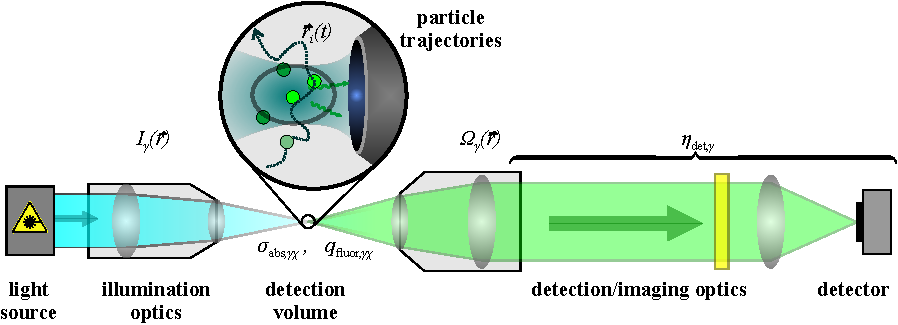
\includegraphics{pic/fcs_microscopeschematic.pdf}
	\mycaption{Schematic of the optics model used for the derivation of FCS theory.}{The illumination optics focuses light into an intensity distribution $I_\gamma(\vr)$. The detection optics is characterized by its detection probability distribution $\Omega_\gamma(\vr)$ and the detection efficiency $\etadetgamma$. The sample is modeled as a set of particles with trajectories $\vr_i(t)$. To each species an absorption cross-section $\sigmaabsgammachi$ and a fluorescence quantum efficiency $\qfluorgammachi$ is assigned. }
  %The microscope is split into its functional components: The light source and illumination optics (illumination profile $I_\gamma(\vr)$), the detection optics (detection probability distribution $\Omega_\gamma(\vr)$) and the detector itself (detection efficiency $\etadetgamma$, summarizing the detector and the detection  optics). The color channel is encoded by the index $\gamma$. The sample itself is modeled as a set of particles $i$ of species $\chi$, following trajectories $\vr_i(t)$. To each species a absorption crosssection $\sigmaabsgammachi$ and a fluorescence quantum efficiency $\qfluorgammachi$ is assigned.}
	\label{fig:fcs_microscopeschematic}
\end{figure}

%In order to 
The theoretical framework of FCS starts from a simplified model of the fluorescence microscope, which is used to acquire the data. \Figref{fig:fcs_microscopeschematic} illustrates this model. It will be explained in detail throughout this section.

The sample of volume $\Vsample$ contains $\Nsamplechi$ particles of species $\chi$ that move randomly. The motion of each particle $i=1...\Nsample(\chi)$ is described by its trajectory $\vr_i(t)$. The trajectories are typically not known exactly, but their statistics, such as the \itindex{mean squared displacement (MSD)}\index{MSD}, is known. Finally, the local particle concentration distribution of species $\chi$ can be written as
\begin{equation}\label{eq:fcstheory_concentration}
  c_\chi(\vr,t)=\frac{1}{\Vsample}\cdot\sum\limits_{i=1}^{\Nsamplechi}\ddelta\bigl[\vr-\vr_i(t)\bigr].
\end{equation}

The particles are illuminated by some kind of illumination optics (e.g. a \itindex{confocal microscope} or a \itindex{selective plane illumination microscope (SPIM)}\index{SPIM}) with an intensity distribution $I_\gamma(\vr)$. The index $\gamma\in\{\txt{g},\txt{r}, ...\}$ denotes the color channel of the microscope, e.g. $\gamma=\txt{g}$ for excitation at $488\unit{nm}$ and detection in the range of $[500...550]\unit{nm}$ to observe eGFP, or $\gamma=\txt{r}$ for excitation at $568\unit{nm}$ and detection at $[600...700]\unit{nm}$ for mRFP. An absorption cross-section $\sigmaabsgammachi$ and a fluorescence quantum yield $\qfluorgammachi$ is assigned to each species. Then the amount of fluorescence emitted by a single fluorophore of species $\chi$ at position $\vr$ into channel $\gamma$ can be written as
  \[ I_\gamma(\vr)\cdot\sigmaabsgammachi\cdot\qfluorgammachi. \]
The detection optics is described by a detection efficiency distribution $\Omega_\gamma(\vr)$ and a detection efficiency $\etadetgamma$. The latter summarizes any signal loss due to optical surfaces or filters in the detection beam path. The distributions $I_\gamma(\vr)$ and $\Omega_\gamma(\vr)$ are not observable independently, so they are usually combined into a single function, called \itindex{molecular detection efficiency (MDE)}\index{MDE}:
\begin{equation}\label{eq:fcstheory_mde}
  \MDE_\gamma(\vr):=I_\gamma(\vr)\cdot\Omega_\gamma(\vr).
\end{equation}
This function is proportional to the rate of fluorescence photons expected from a fluorophore at position~$\vr$. Its actual form for a given microscopy setup can be calculated from the PSFs of the microscope. The geometry of the detectors (e.g. square pixels of a camera) also may need to be taken into account. For confocal setups a 3-dimensional, rotationally symmetric Gaussian function with width $w_\gamma$ and height $z_\gamma$ is a good approximation:
\begin{equation}\label{eq:fcstheory_mde_confocal}
  \MDE_{\txt{confocal,} \gamma}(\vr)=I_0\cdot\exp\left(-2\cdot\frac{x^2+y^2}{w_\gamma^2}-2\cdot\frac{z^2}{z_\gamma^2}\right).
\end{equation}



In Refs.~\cite{WOHLAND2010,SINGHKRIEGER2013,KRIEGERPHD2014} it is argued, that a properly designed and aligned SPIM has a PSF with negligible sidelobe contributions. So the PSF can also be approximated by a Gaussian function. Still the finite size of the quadratic camera pixel has to be taken into account for the final form of the MDE:
\begin{equation}\label{eq:fcstheory_mde_SPIM_int}
  \MDE_{\txt{SPIM,} \gamma}(\vr)=I_0\cdot (h_\txt{pixel}\conv\PSF_{\txt{SPIM,} \gamma})(\vr)=\iint\limits_{-\pixelsize/2\ \ }^{\ \ \pixelsize/2} \PSF_{\txt{SPIM,} \gamma}(\vr-\vr')\;\ddxs\;\ddys,
\end{equation}
where $\pixelsize$ is the width of the pixel in the object plane, $\conv$ denotes convolution and $h_\txt{pixel}(\vr)$ is the characteristic function, describing a camera pixel:
\begin{equation}\label{eq:imaging_CEF}
  h_\txt{pixel}(\vr)=\ddelta(z)\cdot\begin{cases}1 & -\frac{\pixelsize}{2}\leq x\leq\frac{\pixelsize}{2}\ \ \ \wedge\ \ \ -\frac{\pixelsize}{2}\leq y\leq\frac{\pixelsize}{2}\\ 0 & \text{else}\end{cases}.
\end{equation}
The convolution integral in \eqref{eq:fcstheory_mde_SPIM_int} can be solved analytically:
\begin{equation}\label{eq:fcstheory_mde_SPIM}
 \MDE_{\txt{SPIM,} \gamma}(\vr)=I_0\cdot\frac{\left[\erf\left(\frac{\pixelsize-2x}{\sqrt{2}\cdot w_\gamma}\right)+\erf\left(\frac{\pixelsize+2x}{\sqrt{2}\cdot w_\gamma}\right)\right]\cdot\left[\erf\left(\frac{\pixelsize-2y}{\sqrt{2}\cdot w_\gamma}\right)+\erf\left(\frac{\pixelsize+2y}{\sqrt{2}\cdot w_\gamma}\right)\right]}{\left[2\cdot\erf\left(\frac{\pixelsize}{\sqrt{2}\cdot w_\gamma}\right)\right]^2}\cdot\exp\left(-2\cdot\frac{z^2}{z_\gamma^2}\right)
\end{equation}
As shown in \figref{fig:pixel_psf_cut}, this MDE deviates significantly from a Gaussian function, if $\pixelsize$ is significantly larger than the size $w_\gamma$ of the PSF. 

%Throughout the rest of this chapter, results are typically given in two form. For a Gaussian MDE in \eqref{eq:fcstheory_mde_confocal} and for the SPIM MDE in \eqref{eq:fcstheory_mde_SPIM}.


\begin{figure}[t!]
	\centering
    \begin{gnuplot}[terminal=\defaultgnuplotterminal,terminaloptions=\defaultgnuplotterminalopts{14cm}{5cm},preamble=\defaultgnuplotpreamble]
      set xlabel 'positions $x\unitbs{\mu m}$'
      set ylabel '$\MDE_{\txt{SPIM,} \gamma}(x)$ [A.U.]'
      set samples 500
      #set palette rgb 23,28,3;
      unset colorbox
      set key outside rmargin
      MDE(x,w,a)=(erf((a-2.0*x)/(sqrt(2.0)*w))+erf((a+2.0*x)/(sqrt(2.0)*w)))/(2.0*erf(a/(sqrt(2)*w)))
      G(x,w)=exp(-2.0*x*x/w/w)
      plot [-3.5:3.5][0:1.1] MDE(x,0.5,0.5) title 'SPIM MDE: $a=500\unit{nm}$' with lines lc palette frac 0.0, \
                  MDE(x,0.5,1) title 'SPIM MDE: $a=1000\unit{nm}$' with lines lc palette frac 0.3, \
                  MDE(x,0.5,2) title 'SPIM MDE: $a=2000\unit{nm}$' with lines lc palette frac 0.6, \
                  MDE(x,0.5,4) title 'SPIM MDE: $a=4000\unit{nm}$' with lines lc palette frac 1, \
                  G(x,0.5) title 'Gaussian' with lines lc rgbcolor "red"
    \end{gnuplot}

	\mycaption{Plots of cuts through the MDE of a SPIM in \eqref{eq:fcstheory_mde_SPIM} along one coordinate axis.}{ For all plots, the PSF width was $w_\gamma=500\unit{nm}$.}
	\label{fig:pixel_psf_cut}
\end{figure}

Finally, the results of this section can be combined into the fluorescence time trace expected from a fluorophore concentration $c_\chi(\vr,t)$ (see \eqref{eq:fcstheory_concentration}):
\begin{equation}\label{eq:fcstheory_fluorescence_raw}
  F_\gamma(t)=\fullvolint\MDE_\gamma(\vr)\cdot\sum\limits_{\chi\in\bbS}\etadetgamma\cdot\sigmaabsgammachi\cdot\qfluorgammachi\cdot c_\chi(\vr,t)\;\ddV.%\etagammachi
\end{equation}
The factors $\etadetgamma$, $\sigmaabsgammachi$ and $\qfluorgammachi$ are not distinguishable in a FCS experiment, so they are summarized into a single detection efficiency $\etagammachi$ of a fluorophore of species $\chi\in\bbS$ in channel $\gamma$:
\begin{equation}\label{eq:fcstheory_etagammachi}
  \etagammachi\equiv\etadetgamma\cdot\sigmaabsgammachi\cdot\qfluorgammachi
\end{equation}
Then \eqref{eq:fcstheory_fluorescence_raw} can be simplified to
\begin{equation}\label{eq:fcstheory_fluorescence}
  F_\gamma(t)=\fullvolint\MDE_\gamma(\vr)\cdot\sum\limits_{\chi\in\bbS}\etagammachi\cdot c_\chi(\vr,t)\;\ddV.
\end{equation}
As shown in \eqref{eq:fcs_acf}, the autocorrelation function is written in terms of signal fluctuations $\delta F_\gamma(t)$ around a mean intensity $\smean{F_\gamma}$. These can be expressed in a form analogous to \eqref{eq:fcstheory_fluorescence}, if the concentration dynamics $c_\chi(\vr,t)$ is also split into a fluctuation part and  an average concentration:%,  constant over the size of the MDE and the time of the measurement:
\begin{equation}\label{eq:fcstheory_concfluc}
  c_\chi(\vr,t)=\smean{c_\chi}+\delta c_\chi(\vr,t).
\end{equation}
Due to the linearity of \eqref{eq:fcstheory_fluorescence}, this finally yields:
\begin{equation}\label{eq:fcstheory_fluorescencefluc}
  \delta F_\gamma(t)=\fullvolint\MDE_\gamma(\vr)\cdot\sum\limits_{\chi\in\bbS}\etagammachi\cdot \delta c_\chi(\vr,t)\;\ddV.
\end{equation}
%The mean fluorescence signal can be simplified to:
%\begin{equation}\label{eq:fcstheory_meanfluorescence}
%  \mean{F_\gamma}= \sum\limits_{\chi\in\bbS}\etagammachi\fullvolint\MDE_\gamma(\vr)\cdot \mean{c_\chi(\vr)}\;\ddV,= \sum\limits_{\chi\in\bbS}\etagammachi \mean{N_\chi},
%\end{equation}
%where $\smean{N_\chi}$ is the mean number of particles of species $\chi$ in the focal volume, defined by the MDE. In this form the meaning of $\etagammachi$ is simply molecular brightness, i.e. the average amount of fluorescence emitted a single particle of species $\chi$ int the observation volume. 


%Also the MDE is required to be normalized:
%\begin{equation}\label{eq:fcstheory_mde_normalized}
%  \fullvolint\MDE_{\gamma}(\vr)\;\ddV\overset{!}{=}1.
%\end{equation}
%This normalization condition will be used throughout the rest of this thesis, as it simplifies some derivations. As all correlation functions are normalized to the average intensity, the global normalization factor imposed by \eqref{eq:fcstheory_mde_normalized} will not influence the final results. Care has to be taken in order to interpret all other properties are accordingly.



\section{Theory of fluorescence correlation spectroscopy}
\label{sec:ConfocalFluorescenceCorrelationSpectroscopy}
\subsection{The FCS autocorrelation function}
\label{sec:TheFCSAutocorrelationFunctionTheory}


\noindent For a color channel $\gamma$, the FCS autocorrelation function is defined as
\begin{equation*}
  g_\gamma(\tau)=\frac{\mean{\delta F_\gamma(t)\cdot\delta F_\gamma(t+\tau)}}{\mean{F_\gamma}^2}. \tag{\ref{eq:fcs_acf}}
\end{equation*}
Using the results in \eqsref{eq:fcstheory_fluorescence}{eq:fcstheory_fluorescencefluc} this can be rewritten as:
\begin{equation}\label{eq:fcs_acffull}
  g_\gamma(\tau)=\frac{\sum\limits_{\chi\in\bbS}\etagammachi^2 \fullvolint\fullvolint\MDE_\gamma(\vr)\cdot\MDE_\gamma(\vr')\cdot\mean{\delta c_\chi(\vr,t)\cdot\delta c_\chi(\vr',t+\tau)}\;\ddV\ddV' }{\left(\sum\limits_{\chi\in\bbS}\etagammachi \cdot\fullvolint\MDE_\gamma(\vr)\cdot \mean{c_\chi(\vr,t)}\;\ddV\right)^2}.
\end{equation}
Here, the linearity of the integration and averaging $\smean{\cdot}$ was used. Furthermore, it was assumed that the concentration fluctuations from two different molecular species $\chi$ and $\chi'$ are statistically independent, i.e. $\smean{\delta c_\chi(\vr,t)\cdot\delta c_{\chi'}(\vr,t)}=0$.

\subsection{Zero-lag correlation and particle numbers}
\label{sec:ZeroLagCorrelationAndEffectiveVolume}
%As a first result, an extended form of the statement in \eqref{eq:fcs_acfn} on the zero-lag amplitude of the autocorrelation function $g(0)\propto 1/\mean{N}$ can be made, using again 
The Poissonian nature of the particle number (or concentration) in the focus dictates for $\tau=0$:
\begin{equation}\label{eq:fcs_zerolagconcentrationcorrelation}
  \mean{\delta c_\chi(\vr,t)\cdot\delta c_\chi(\vr',t)}\equiv\mean{\delta c_\chi^2(\vr,t)}\cdot\ddelta(\vr-\vr')=\mean{c(\vr,t)}\cdot\ddelta(\vr-\vr'),
\end{equation}
where the factor $\ddelta(\vr-\vr')$ signifies, that single particles are non-interacting and therefore, also statistically independent. Therefore they are only correlated to themselves and not to other particles nearby. 
Using \eqref{eq:fcs_zerolagconcentrationcorrelation} and further assuming that the concentration does not change significantly over the observation volume (described by the MDE), i.e. $\smean{c_\chi(\vr)}\equiv\smean{c_\chi}$, the zero-lag autocorrelation amplitude becomes: %\eqref{eq:fcs_acffull} can be further simplified for $\tau=0$:
\begin{multline}\label{eq:fcs_acffull_zerolag}
  g_\gamma(0)=\frac{\sum\limits_{\chi\in\bbS}\etagammachi^2\cdot\smean{c_\chi}\cdot \fullvolint\MDE_\gamma^2(\vr)\;\ddV }{\left(\sum\limits_{\chi\in\bbS}\etagammachi \cdot\smean{c_\chi}\cdot\fullvolint\MDE_\gamma(\vr)\;\ddV\right)^2}=\\
  =\frac{\sum\limits_{\chi\in\bbS}\etagammachi^2\cdot\smean{c_\chi} }{\left(\sum\limits_{\chi\in\bbS}\etagammachi \cdot\smean{c_\chi}\right)^2}\cdot\frac{\fullvolint\MDE_\gamma^2(\vr)\;\ddV}{\left(\fullvolint\MDE_\gamma(\vr)\;\ddV\right)^2}\underset{\bbS=\{\chi\}}{=} \frac{1 }{\smean{c_\chi}}\cdot\frac{\fullvolint\MDE_\gamma^2(\vr)\;\ddV}{\left(\fullvolint\MDE_\gamma(\vr)\;\ddV\right)^2}.
\end{multline}
In the last step, a single species $\chi$ was assumed. %If the last fraction in this result is interpreted as an inverse volume, i.e.
Introducing the effective volume %$\Veffm{\gamma}$
\begin{equation}\label{eq:fcs_Veff}
  \Veffm{\gamma}:=\frac{\left(\fullvolint\MDE_\gamma(\vr)\ddV\right)^2}{\fullvolint\MDE_\gamma^2(\vr)\ddV}
\end{equation}
 of the MDE, the zero-lag amplitude of the autocorrelation function can be written in terms of a particle number $\smean{N_\chi}=\smean{c_\chi}\cdot\Veffm{\gamma}$ within this volume:
\begin{equation}\label{eq:fcs_acf_zerolag}
  g_\gamma(0)=\frac{\sum\limits_{\chi\in\bbS}\etagammachi^2\cdot\smean{c_\chi}\cdot\Veffm{\gamma} }{\left(\sum\limits_{\chi\in\bbS}\etagammachi \cdot\smean{c_\chi}\cdot\Veffm{\gamma}\right)^2} =\frac{\sum\limits_{\chi\in\bbS}\etagammachi^2\cdot\mean{N_\chi} }{\left(\sum\limits_{\chi\in\bbS}\etagammachi \cdot\mean{N_\chi}\right)^2}\underset{\bbS=\{\chi\}}{=}\frac{1}{\mean{N_\chi}}.
\end{equation}

For confocal and light sheet microscopes, the MDEs were defined in section \ref{sec:FCSModelingTheOpticalSystem}. The integrals in the effective volume in \eqref{eq:fcs_Veff} can be calculated analytically for these specific MDEs:
\begin{align}
   \text{confocal:} \ \ \ \ \ \ \Veffm{\gamma}&=\pi^{3/2}\cdot w_\gamma^2\cdot z_\gamma,\label{eq:fcs_Veff_confocal}\\
   \text{SPIM:} \ \ \ \ \ \ \Veffm{\gamma}&= \frac{\sqrt{\pi}\cdot \pixelsize^{2}\cdot z_\gamma}{\left[\erf\left(\frac{\pixelsize}{w_\gamma}\right)+\frac{w_\gamma}{\sqrt\pi\cdot \pixelsize}\left(\ee^{-\pixelsize^2/w_{\gamma}^2}-1\right)\right]^2}.\label{eq:fcs_Veff_SPIM}
\end{align}


\subsection{The concentration correlation factor}
\label{sec:TheConcentrationCorrelationFactor}
\noindent In the autocorrelation function \eqref{eq:fcs_acffull} the particle dynamics is fully described by the concentration correlation factor 
\begin{equation}\label{eq:fcs_corrfactordef}
    \mean{\delta c_\chi(\vr,t)\cdot\delta c_\chi(\vr',t+\tau)}=:\phi_\chi(\vr,\vr',\tau)\equiv \phi_\chi(\vr-\vr',\tau).
\end{equation}
It quantifies the amount of correlation at a time-lag $\tau$ between the concentration fluctuations at two positions $\vr$ and $\vr'$. The last equivalence in \eqref{eq:fcs_corrfactordef} states that $\phi_\chi(\cdot,\cdot)$ only depends on the difference in positions, i.e. the whole system is shift-invariant in space. If the system of interest is furthermore isotropic, the self correlation function only depends on the length $\snorm{\vr-\vr'}$, i.e. \mbox{$\phi_\chi(\vr,\vr',\tau)\equiv \phi_\chi(\snorm{\vr-\vr'},\tau)$}. Note that generally these assumptions are not necessarily true, but on the small scales of FCS measurements they usually are assumed to apply.

%As stated in \eqref{eq:fcs_zerolagconcentrationcorrelation}, initially ($\tau=0$) correlation has not spread over space yet and thus the correlation factor is proportional to $\ddelta(\vr-\vr')$. For an arbitrary time lag $\tau$, it has to be calculated from the equations of motion of the modeled system, e.g. the diffusion differential equation \deqref{eq:intro_diffusion_dgl}.

The concentration correlation factor is (up to prefactors) equivalent to the van-Hove self correlation function of the particles \cite{HANSEN2013,HOPKIN2010,HOFLIN2013}, which is given in terms of single-particle trajectories $i=1,2,...,N$ as \cite{HOPKIN2010}:
\begin{align}\label{eq:fcs_vanhove_trajectory}
    P_\chi(\vr,\vr',\tau)&=\frac{1}{N}\cdot\mean{\sum\limits_{i=1}^N\ddelta(\vr'-\vr+\vr_i(0)-\vr-(\vr_i(\tau)-\vr)}.
\end{align}
Here, $P_\chi(\cdot,\cdot,\cdot)$ can be interpreted as the probability to find a particle at position $\vr'$ at time $\tau$, if it was initially at position $\vr$. Specific forms of $P_\chi(\cdot,\cdot)$ can be calculated as the Green's function or propagator of the \itindex{photon detection efficiency (PDE)}\index{PDE}, which governs the dynamics of $c_\chi(\vr,t)$. A simple example for the PDE is the \itindex{diffusion equation} in 
  \begin{equation}\label{eq:intro_diffusion_dgl}  
    \fracpd{c(\vr, t)}{t}= D\cdot \vnabla^2c(\vr, t),
  \end{equation}
where $D$ is the \itindex{diffusion coefficient}.
%In that framework, $\phi_\chi(\cdot,\cdot)$ equals the Green's function, or propagator $P_\chi(\vr,\vr',\tau)$ of the PDE. 
The Green's function is defined as the solution of the PDE for the initial condition $c_\chi(\vr,0)=\ddelta(\vr)$ \cite{BOAS1983}. It can be used to calculate the solution $c_\chi(\vr,\tau)$ of the PDE for an arbitrary initial condition $c_\chi(\vr,0)$ at any time $\tau>0$:
\begin{equation}\label{eq:intro_diffusion_dgl_solution_greens}  
  c_\chi(\vr,\tau)=c_\chi(\vr,0)\conv P_\chi(\vr,\tau)=\idotsint c_\chi(\vr',0)\cdot P_\chi(\vr,\vr',\tau)\;\dd^\ddim r'.
\end{equation}
Here $\conv$ denotes a convolution and $\ddim$ is the dimension of the space, in which the motion takes place. Finally, the concentration correlation factor is given by
\begin{equation}\label{eq:fcs_diffusion_vanHove_and_Propagator}  
  \phi_\chi(\vr,\vr',\tau)=\mean{\delta c_\chi(\vr,t)\cdot\delta c_\chi(\vr',t+\tau)}=\smean{c_\chi}\cdot P_\chi(\vr,\vr',\tau).
\end{equation}


\noindent With these definitions, \eqref{eq:fcs_acffull} can be slightly rewritten:
\begin{multline}\label{eq:fcs_acffull_phifactor}
  g_\gamma(\tau)=\frac{\sum\limits_{\chi\in\bbS}\etagammachi^2 \smean{c_\chi}\fullvolint\fullvolint\MDE_\gamma(\vr)\cdot\MDE_\gamma(\vr')\cdot\phi_\chi(\vr,\vr',\tau)\;\ddV\ddV' }{\left(\sum\limits_{\chi\in\bbS}\etagammachi \smean{c_\chi}\right)^2\cdot\left(\fullvolint\MDE_\gamma(\vr)\;\ddV\right)^2}=\\
  =\frac{\sum\limits_{\chi\in\bbS}\etagammachi^2 G_{\gamma}^{\chi}(\tau) }{\left(\sum\limits_{\chi\in\bbS}\etagammachi \smean{c_\chi}\right)^2}.
\end{multline}
In this form a non-normalized correlation function
\begin{multline}\label{eq:fcs_nnormacf}
  G_{\gamma}^{\chi}(\tau):=\frac{\mean{\delta F_\gamma^{\chi}(t)\cdot\delta F_\gamma^{\chi}(t+\tau)}}{\etagammachi^2\cdot\left(\fullvolint\MDE_\gamma(\vr)\;\ddV\right)^2}=\\
  =\smean{c_\chi}\cdot\frac{\fullvolint\fullvolint\MDE_\gamma(\vr)\cdot\MDE_\gamma(\vr')\cdot\phi_\chi(\vr,\vr',\tau)\;\ddV\ddV'}{\left(\fullvolint\MDE_\gamma(\vr)\;\ddV\right)^2}
\end{multline}
of the fluctuations $\delta F_\gamma^{\chi}(t)$ caused by a single species $\chi$ in a channel $\gamma$ is introduced.


%Now the problem of calculating the FCS autocorrelation function for a given situation is reduced to finding the van-Hove self correlation function. In many cases, the dynamics is governed by a linear (partial) differential equation. Then its solution $\delta c_\chi(\vr,t+\tau)$ is given by the Green's function or propagator $P(\vr,\vr',\tau)$ of the equations of motion and an initial condition $\delta c_\chi(\vr,t)$ \cite{BOAS1983}:
  %\[ \delta c_\chi(\vr,t+\tau)=\delta c_\chi(\vr,t)\conv P(\vr,\vr', \tau) \]
%In that case the van Hove self correlation function is generally given by:
%\begin{equation}\label{eq:fcs_diffusion_vanHove_and_Propagator}  
  %\phi_\chi(\vr,\vr',\tau)=\mean{\delta c_\chi(\vr,t)\cdot\delta c_\chi(\vr',t+\tau)}=\smean{c_\chi}\cdot P_\chi(\vr,\vr',\tau).
%\end{equation}
%This result can be derived, using that in reciprocal Fourier space (see appendix~\ref{sec:FourierTransform}) the convolution translates to a multiplication:
%\begin{align*}
  %\phi_\chi(\vr,\vr',\tau)&=\mean{\delta c_\chi(\vr,t)\cdot\delta c_\chi(\vr',t+\tau)}=\mean{\delta c_\chi(\vr,t)\cdot\left[\delta c_\chi(\vr',t)\conv P(\vr,\vr',\tau)\right]}=\\
  %&=\mean{\FTia[\vk']{\delta c_\chi(\vr,t)\cdot\delta \tilde c_\chi(\vk',t+\tau)}}=\FTia[\vk']{\mean{\delta c_\chi(\vr,t)\cdot\delta \tilde c_\chi(\vk',t)}\cdot\tilde P_\chi(\vr,\vk',\tau)}=\\
  %&=\mean{\delta c_\chi(\vr,t)\cdot\delta c_\chi(\vr',t)}\conv P_\chi(\vr,\vr',\tau)
%\end{align*}
%Here $\tilde{f}(\vk)$ is the Fourier transform of a function $f(\vr)$ and $f(\vr)=\FTia[\vk]{\tilde f(\vk)}$ denotes inverse Fourier transform. Linearity of Fourier transform and averaging allows one to exchange the two operations. Note in the second line, that the factor $\tilde P_\chi(\vr,\vk',\tau)$ does not depend on the absolute time $t$, so it can be written outside the time-average $\mean{\cdot}$. Finally using the $\ddelta$-function in \eqref{eq:fcs_zerolagconcentrationcorrelation}, the last line of equations can be rewritten in a simple form:
%\begin{equation*}
  %\phi_\chi(\vr,\vr',\tau)=\mean{\delta c_\chi(\vr,t)\cdot\delta c_\chi(\vr',t+\tau)}=\smean{c_\chi}\cdot P_\chi(\vr,\vr',\tau).\tag{\ref{eq:fcs_diffusion_vanHove_and_Propagator}  }
%\end{equation*}
%This result was derived, starting from the diffusion equation, but it is generally true, as long as $\delta c_\chi(\vr,t+\tau)$ can be written as a convolution of $\delta c_\chi(\vr,t)$ with a propagator $P(\vr,\vr',\tau)$, because the actual form of the diffusion equation was never used.

The next subsections will give the exact mathematical form of $\phi_\chi(\vr,\vr',\tau)$ and the FCS autocorrelation functions $G_{\gamma}^{\chi}(\tau)$ and $g(\tau)$ for different situations frequently encountered in FCS measurements.



\subsection{Normal diffusion}\index{normal diffusion}\index{diffusion}
\label{sec:NormalDiffusionFCS}
The most common dynamics in FCS is normal diffusion. Here, the particle concentration dynamics $c_\chi(\vr,t)=\smean{c_\chi}+\delta c_\chi(\vr,t)$ is governed by the \itindex{diffusion equation} \eqref{eq:intro_diffusion_dgl}:
\begin{equation}\label{eq:fcs_diffusion_dgl_fluctuations}  
  \fracpd{\left(\smean{c_\chi}+\delta c_\chi(\vr, t)\right)}{t}=D_\chi\cdot \vnabla^2\left(\smean{c_\chi}+\delta c_\chi(\vr, t)\right)\ \ \ \ \ \Rightarrow\ \ \ \ \ \ \fracpd{\delta c_\chi(\vr, t)}{t}=D_\chi\cdot \vnabla^2\delta c_\chi(\vr, t).
\end{equation}
The Green's function of the this PDE \eqref{eq:fcs_diffusion_dgl_fluctuations} is
\begin{equation}\label{eq:fcs_ndiff_propagator}
  P_\chi(\vr,\vr',\tau)=\frac{1}{\Bigl(4\pi D_\chi\tau\Bigr)^{3/2}}\cdot\exp\left(-\frac{(\vr'-\vr)^2}{4D_\chi\tau}\right).
\end{equation}
Note that the \itindex{diffusion equation} \eqref{eq:intro_diffusion_dgl} (and likewise \eqref{eq:fcs_diffusion_dgl_fluctuations}) can be interpreted statistically and then also a single-particle \itindex{mean squared displacement (MSD)} can be calculated. For normal diffusion in $d$ dimensions, Albert Einstein derived:
\begin{equation}\label{eq:msd_normal_diffusion}
  \MSD(\tau)\equiv\langle r^2\rangle(\tau)=2d\cdot D\cdot\tau.
\end{equation}


%Using this, the FCS autocorrelation functions can be calculated analytically from \eqref{eq:fcs_nnormacf}, provided that the MDE is sufficiently. Especially in the case of the MDEs given in \eqref{eq:fcs_Veff_confocal} and \eqref{eq:fcs_Veff_SPIM}, the volume integrals separate into three independent coordinate directions, so the non-normalized correlation function reads:
With this result and the MDEs in \eqsref{eq:fcs_Veff_confocal}{eq:fcs_Veff_SPIM}, the FCS autocorrelation function for normal diffusion can be calculated. The MDEs as well as \eqref{eq:fcs_ndiff_propagator} can be separated into three factors that depend solely on a single direction $x$, $y$ or $z$. Therefore, also the autocorrelation function separates into three directional components:
\begin{equation}\label{eq:fcs_ndiff_cc_separated}
  G_{\gamma}^{\chi}(\tau)=\smean{c_\chi}\cdot G_{\gamma,x}^{\chi}(\tau)\cdot G_{\gamma,y}^{\chi}(\tau)\cdot G_{\gamma,z}^{\chi}(\tau).
\end{equation}
Each directional factor is defined by
\begin{equation}\label{eq:fcs_ndiff_cc_separated_dirfactor}
   G_{\gamma,x}^{\chi}(\tau)=\frac{\int\limits_{-\infty}^\infty\int\limits_{-\infty}^\infty\MDE_{\gamma,x}(\xi)\cdot\MDE_{\gamma,x}(\xi')\cdot\phi_{\chi,x}(\xi,\xi',\tau)\dd\xi\dd\xi'}{\left(\int\limits_{-\infty}^\infty\MDE_x(\xi)\dd\xi\right)^2}.
\end{equation}
Here the directional components of $\MDE_\gamma(\vr)$ and of  $\phi_\chi(\vr,\vr',\tau)$ are denoted by an additional index $x$.


For a 3-dimensional Gaussian MDE (\eqrefn{eq:fcstheory_mde_confocal}), the directional factor in \eqref{eq:fcs_ndiff_cc_separated_dirfactor} is given for the $x$ and $y$ direction by%for directions $x$ or $y$ with the associated MDE-width $w_\gamma$ (or $z$ with width $z_\gamma$ by replacement) is
\begin{equation}\label{eq:fcs_ndiff_cc_confocal_separated_factor}
  G_{\gamma,x}^{\chi}(\tau)=\frac{1}{\sqrt{\pi}\cdot w_\gamma}\cdot\left(1+\frac{4D_\chi\tau}{w_\gamma^2}\right)^{-1/2}.
\end{equation}
The factor for the $z$ direction is of the same form, but with $w_\gamma$ replaced by  $z_\gamma$.
From this the non-normalized correlation function is easily calculated:
\begin{equation}\label{eq:fcs_ndiff_cc_confocal}
  G_{\gamma}^{\chi}(\tau)=\frac{\smean{c_\chi}}{\pi^{3/2}w_\gamma^2 z_\gamma}\cdot\left(1+\frac{4D_\chi\tau}{w_\gamma^2}\right)^{-1}\cdot\left(1+\frac{4D_\chi\tau}{z_\gamma^2}\right)^{-1/2}.
\end{equation}
The final FCS normalized correlation function is then given by:
\begin{equation}\label{eq:fcs_ndiff_confocal}
  g_{\gamma}(\tau)=\frac{1}{\smean{c_\chi}\cdot\pi^{3/2}w_\gamma^2 z_\gamma}\cdot\left(1+\frac{4D_\chi\tau}{w_\gamma^2}\right)^{-1}\cdot\left(1+\frac{4D_\chi\tau}{z_\gamma^2}\right)^{-1/2},
\end{equation}
which can be reformulated to
\begin{equation}\label{eq:fcs_ndiff_confocal_NTauD}
  g_{\gamma}(\tau)=\frac{1}{\smean{N_\chi}}\cdot\left(1+\frac{\tau}{\tauDm{\chi}}\right)^{-1}\cdot\left(1+\frac{\tau}{(z_\gamma/w_\gamma)^2\cdot\tauDm{\chi}}\right)^{-1/2}.
\end{equation}
Here $\smean{N_\chi}$ is the average number of particles in a focal volume as given by \eqref{eq:fcs_Veff_confocal} and $\tauDm{\chi}$ is the diffusion correlation time with
\begin{equation}\label{eq:fcs_ndiff_confocal_tauD}
  \tauDm{\chi}=\frac{w_\gamma^2}{4D_\chi}.
\end{equation}
This $\tauDm{\chi}$ is the average dwell time of particles in the observation volume and also the half decay time of $g_\gamma(\tau)$. \Figref{fig:fcs_confocal_acf_3ddiff_confocal} illustrates the function $g_\gamma(\tau)$ for a single species $\chi$ for different the diffusion coefficients and the particle numbers. The red lines in \figrefs{fig:fcs_confocal_acf_3ddiff_confocal}{a} indicate $\tauDm{\chi}$ for the different cases. They demonstrate that $g_\gamma(\tauDm{\chi}) =g_\gamma(0)/2$. \Figrefs{fig:fcs_confocal_acf_3ddiff_confocal}{b} illustrates the general dependence $g_\gamma(0)=1/\smean{N_\chi}$ of the zero-lag amplitude on the average particle number $\smean{N_\chi}$ in the focal volume.


\begin{figure}[t!]
	\centering
	\begin{minipage}{164mm}\small
		\begin{minipage}{82mm}(a)\\[-3mm]
			\begin{gnuplot}[terminal=\defaultgnuplotterminal,terminaloptions=\defaultgnuplotterminalopts{8cm}{6cm},preamble=\defaultgnuplotpreamble]
			  set format x '\footnotesize $10^{%T}$';
        w=0.25
        gamma=6
        N=10
        tD(D)=w*w/4.0/D
			  g(tau, tauD, N, gamma)=1.0/(1.0+tau/tauD)/sqrt(1.0+tau/tauD/gamma/gamma)/N
			  set logscale x
			  set xlabel 'lag time $\tau\unitb{s}$'
			  set ylabel 'correlation amplitude $g_\gamma(\tau)$'
        #set palette rgb 23,28,3;
        unset colorbox
        set key inside right top vertical  opaque  maxrows 3
        set arrow from 1e-6,g(1,1,N,gamma) to tD(1),g(1,1,N,gamma) nohead fc rgbcolor "light-red"
        set arrow from tD(1),g(1,1,N,gamma) to tD(1),0 nohead fc rgbcolor "light-red"
        set arrow from tD(10),g(1,1,N,gamma) to tD(10),0 nohead fc rgbcolor "light-red"
        set arrow from tD(100),g(1,1,N,gamma) to tD(100),0 nohead fc rgbcolor "light-red"

			  plot [1e-6:10][0:0.105] g(x, tD(100),N,gamma) title '\footnotesize $D_\chi=100\unit{\mu m^2/s}$' with lines lc palette frac 0,  \
                      g(x, tD(10),N,gamma) title '\footnotesize $D_\chi=10\unit{\mu m^2/s}$' with lines lc palette frac 0.5,  \
                      g(x, tD(1),N,gamma) title '\footnotesize $D_\chi=1\unit{\mu m^2/s}$' with lines lc palette frac 1 
			\end{gnuplot}
	  \end{minipage}
		\begin{minipage}{82mm}(b)\\[-3mm]
			\begin{gnuplot}[terminal=\defaultgnuplotterminal,terminaloptions=\defaultgnuplotterminalopts{8cm}{6cm},preamble=\defaultgnuplotpreamble]
			  set format x '\footnotesize $10^{%T}$'; 
        w=0.25
        gamma=6
        D=10
        tD(D)=w*w/4.0/D
			  g(tau, tauD, N, gamma)=1.0/(1.0+tau/tauD)/sqrt(1.0+tau/tauD/gamma/gamma)/N
			  set logscale x
			  set xlabel 'lag time $\tau$ [s]'
			  set ylabel 'correlation amplitude $g_\gamma(\tau)$'
        set key inside right top vertical  opaque width +1 maxrows 3
        #set palette rgb 23,28,3;
        unset colorbox
			  plot [1e-6:10][0:0.21] g(x, tD(D),5,gamma) title '\footnotesize $\langle{N_\chi}\rangle=5$' with lines lc palette frac 0,  \
                      g(x, tD(D),10,gamma) title '\footnotesize $\langle{N_\chi}\rangle=10$' with lines lc palette frac 0.5,  \
                      g(x, tD(D),15,gamma) title '\footnotesize $\langle{N_\chi}\rangle=15$' with lines lc palette frac 1
			\end{gnuplot}
	  \end{minipage}
  \end{minipage}
	\mycaption{Plots of the autocorrelation function for a confocal microscope and 3-dimensional normal diffusion, as defined in \eqref{eq:fcs_ndiff_confocal}.}{In (a) the diffusion coefficient is varied, whereas in (b) the average particle number changes. In (a) the red lines indicate the diffusion correlation time $\tauDm{\chi}$ as defined by \eqref{eq:fcs_ndiff_confocal_tauD} for each of the curves. Fixed parameters: $\smean{N_\chi}=10$, $D_\chi=100\unit{\mu m^2/s}$; MDE parameters: $w_\gamma=250\unit{nm}$, $\kappa_\gamma=6$.}
	\label{fig:fcs_confocal_acf_3ddiff_confocal}
\end{figure}


\paragraph{Lower-dimensional diffusion:} Using the separation of the confocal FCS autocorrelation function into directional components, also lower-dimensional diffusion models are easy to set up. 
In \eqref{eq:fcs_ndiff_cc_separated_dirfactor} one can easily omit the dimensions, along which no motion takes place. 
The concentrations $\smean{c_\chi}$ then have to be reinterpreted as an areal density, or a line density, depending on the diffusion model.



\begin{figure}[t!]
	\centering
  \begin{minipage}{164mm}\small
		\begin{minipage}{82mm}(a)\\[-3mm]
			\begin{gnuplot}[terminal=\defaultgnuplotterminal,terminaloptions=\defaultgnuplotterminalopts{8cm}{6cm},preamble=\defaultgnuplotpreamble]
			  set format x '\footnotesize $10^{%T}$';
        N1=5
        N2=5
        w=0.5
        z=1.2
        a=0.4
        c=10
        D2=1
        D11=100
        D12=10
        D13=2
				sqr(x)=x*x
        gg(tau,D,N)=N/(1.0+4.0*D*tau/w/w)/sqrt(1.0+4.0*D*tau/z/z)
        g(tau, D1, D2, N1, N2)=(gg(tau,D1,N1)+gg(tau,D2,N2))/sqr(N1+N2)
        
        fit g(x,Df1,Df1,N1+N2,0) './data/tau.dat' using ($1):(g($1, D11, D2, N1, N2)) via Df1
        fit g(x,Df2,Df2,N1+N2,0) './data/tau.dat' using 1:(g($1, D12, D2, N1, N2)) via Df2
        fit g(x,Df3,Df3,N1+N2,0) './data/tau.dat' using 1:(g($1, D13, D2, N1, N2)) via Df3
        set logscale x
        set xlabel 'lag time $\tau\unitb{s}$'
        set ylabel 'correlation amplitude $g_\gamma(\tau)$'
        #set palette rgb 23,28,3;
        unset colorbox
        set key inside left bottom vertical  opaque  maxrows 4

        plot [1e-5:10][0:0.105] g(x, D2,   D2, N1, N2) title '\footnotesize 1 component' with lines lt 1 lc rgbcolor "black" lw 1,  \
                                g(x, D11,  D2, N1, N2) title '\footnotesize $D_1=100\unit{\mu m^2/s}$' with lines lc palette frac 0,  \
                                g(x, Df1,  Df1, N1+N2, 0) notitle with lines lt 10 lc palette frac 0 lw 2,  \
                                g(x, D12,  D2, N1, N2) title '\footnotesize $D_1=10\unit{\mu m^2/s}$' with lines lc palette frac 0.3,  \
                                g(x, Df2,  Df2, N1+N2, 0) notitle with lines lt 10 lc palette frac 0.3 lw 2,  \
                                g(x, D13,  D2, N1, N2) title '\footnotesize $D_1=2\unit{\mu m^2/s}$' with lines lc palette frac 0.6 ,  \
                                g(x, Df3,  Df3, N1+N2, 0) notitle with lines lt 10 lc palette frac 0.6 lw 2
                                
			\end{gnuplot}
	  \end{minipage}
		\begin{minipage}{82mm}(b)\\[-3mm]
			\begin{gnuplot}[terminal=\defaultgnuplotterminal,terminaloptions=\defaultgnuplotterminalopts{8cm}{6cm},preamble=\defaultgnuplotpreamble]
			  set format x '\footnotesize $10^{%T}$';
        N=10
        N0=0
        N1=N*0.2
        N2=N*0.4
        N3=N*0.6
        N4=N*0.8
        N5=N
        w=0.5
        z=1.2
        a=0.4
        c=10
        D2=1
        D1=100
        Veff=sqrt(pi)*a*a*z/(erf(a/w)+w/sqrt(pi)/a*(exp(-a*a/w/w)-1.0))**2
        Aeff=a*a/(erf(a/w)+w/sqrt(pi)/a*(exp(-a*a/w/w)-1.0))**2
        tD(D)=Aeff/4.0/D
        sqr(x)=x*x
        gg(tau,D,N)=N/Veff/(sqrt(pi)*a*a*z)*sqr(erf(a/sqrt(4*D*tau+w*w))+sqrt(4*D*tau+w*w)/a/sqrt(pi)*(exp(-a*a/(4*D*tau+w*w))-1)) /sqrt(1+4.0*D*tau/z/z)
        g(tau, D1, D2, N1, N2)=(gg(tau,D1,N1)+gg(tau,D2,N2))/sqr(N1/Veff+N2/Veff)
        
        set logscale x
        set xlabel 'lag time $\tau\unitb{s}$'
        set ylabel 'correlation amplitude $g_\gamma(\tau)$'
        
        set key inside right top vertical  opaque  maxrows 6
        set label 1 '$D_1=100\unit{\mu m^2/s}$' at 3e-5,0.02 left front
        set label 2 '$D_2=1\unit{\mu m^2/s}$' at 3e-5,0.01 left front

        plot [1e-5:10][0:0.105] g(x, D1,   D2, N0, N-N0) title '\footnotesize $\rho_1=0\%$' with lines lc palette frac 0,  \
                                g(x, D1,   D2, N1, N-N1) title '\footnotesize $\rho_1=20\%$' with lines lc palette frac 0.2,  \
                                g(x, D1,   D2, N2, N-N2) title '\footnotesize $\rho_1=40\%$' with lines lc palette frac 0.4,  \
                                g(x, D1,   D2, N3, N-N3) title '\footnotesize $\rho_1=60\%$' with lines lc palette frac 0.6,  \
                                g(x, D1,   D2, N4, N-N4) title '\footnotesize $\rho_1=80\%$' with lines lc palette frac 0.8,  \
                                g(x, D1,   D2, N5, N-N5) title '\footnotesize $\rho_1=100\%$' with lines lc palette frac 0.9
			\end{gnuplot}
	  \end{minipage}
  \end{minipage}
	\mycaption{Plots of the confocal FCS autocorrelation function for a two-component system $\chi=1,2$ with $\etam{\gamma}{1}=\etam{\gamma}{2}$, as defined by \eqref{eq:fcs_ndiff_cc_confocal}.}{In (a) one diffusion coefficient is fixed to $D_2=1\unit{\mu m^2/s}$ and $D_1$ is varied, while $\smean{N_1}=\smean{N_2}=5$. The black line is a one-component model with $\mean{N_1}=10$ and $D_1=1\unit{\mu m^2/s}$. The dotted lines represent 1-component fits to the 2-component curves. In (b) the diffusion coefficients are fixed to $D_1=100\unit{\mu m^2/s}$, $D_2=1\unit{\mu m^2/s}$ in all curves, but the particle number fraction $\rho_1:=\smean{N_1}/(\smean{N_1}+\smean{N_2})$ is varied, keeping $\smean{N_1}+\smean{N_2}=10$. MDE parameters: $w_\gamma=500\unit{nm}$, $z_\gamma=1200\unit{nm}$.}
	\label{fig:fcs_confocal_acf_2comp_3ddiff_SPIM}
\end{figure}

\paragraph{Multi-component diffusion:} \Figref{fig:fcs_confocal_acf_2comp_3ddiff_SPIM} shows exemplary autocorrelation curves of a 2-component confocal FCS autocorrelation model. To simplify the situation, the molecular brightnesses of both species $\chi=1,2$ are set equal ($\etam{\gamma}{1}=\etam{\gamma}{2}$). \Figrefs{fig:fcs_confocal_acf_2comp_3ddiff_SPIM}{a} shows a 2-component model with different combinations of diffusion coefficients (solid lines) and 1-component fits (dotted line) to these. The 1-component fit is hardly distinguishable from the 2-component data if the diffusion coefficients are too close to each other. %Typically diffusion coefficients with $D_1/D_2\geq 10$ are easily distinguishable in FCS.
If the assumption of equal brightnesses holds in a system, the multi-component diffusion model is typically written in terms of an overall concentration $\smean{c_\txt{all}}$ and relative concentrations $\rho_\chi$ for each species, with:
\begin{equation}\label{eq:fcs_multicomp_fractions}
    \smean{c_\txt{all}}:=\sum\limits_{\chi\in\bbS}\smean{c_\chi},\ \ \ \ \ \rho_\chi:=\frac{\smean{c_\chi}}{\smean{c_\txt{all}}}\ \ \ \ \ \text{and}\ \ \ \ \ \sum\limits_{\chi\in\bbS}\rho_\chi\overset{!}{=}1.
\end{equation}
With these definition, \eqref{eq:fcs_acffull_phifactor} can be simplified to:
\begin{equation}\label{eq:fcs_acffull_phifactor_relC}
  g_\gamma(\tau)=\frac{1}{\smean{c_\txt{all}}^2}\cdot\sum\limits_{\chi\in\bbS} G_{\gamma}^{\chi}(\tau) 
\end{equation}


